\documentclass[a4paper,12pt]{article}
\usepackage[utf8]{inputenc}
\usepackage{amsmath}
\usepackage{amssymb}
\usepackage{geometry}
\geometry{a4paper, left=1.5cm, right=1.5cm, top=1.5cm, bottom=1.5cm}
\usepackage{titlesec}
\usepackage{titling}
\usepackage{algorithm}
\usepackage{algpseudocode}
\usepackage{graphicx}   
\usepackage{subcaption}
\usepackage{clrscode3e}



\setlength{\droptitle}{-3em}

\titleformat{\section}{\normalfont\large\bfseries}{\thesection}{1em}{}
\titleformat{\subsection}{\normalfont\normalsize\bfseries}{\thesubsection}{1em}{}
\titleformat{\subsubsection}{\normalfont\small\bfseries}{\thesubsubsection}{1em}{}

\title{Alberi AVL}
\author{Francesco Gori}

\begin{document}

\maketitle

\section{Introduzione}
Gli alberi AVL, dal nome dei loro inventori Adelson-Velsky e Landis, sono una classe di alberi binari di ricerca auto-bilancianti simili agli alberi rosso-neri.\\ 
Durante l'inserimento e la cancellazione di nuovi elementi può essere necessario dover fare modifiche all'albero per mantenere l'altezza dell'albero bilanciata; questo fa sì che le operazioni abbiano una complessità temporale specifica.\\
Le operazioni di inserimento, cancellazione, minimo, massimo, successore, predecessore e ricerca si eseguono in tempo $O(lg \, n)$


\section{Proprietà degli Alberi AVL}
Gli elementi di un AVL hanno, oltre agli attributi di un ABR normale, un attributo \textit{h} che ne specifica l'altezza. Questa è definita come il numero di archi nel percorso più lungo dalla radice a una foglia.\\
La proprietà principale degli alberi AVL è che, per ogni nodo, l'altezza dei suoi sottoalberi differisce al massimo di 1. In formule: 
$$|BF(x)| \leq 1 \quad \text{dove} \quad BF(x)=x.left.h-x.right.h$$
\subsection{Altezza Massima e Numero Minimo di Nodi}
L'altezza massima di un AVL con \textit{n} nodi interni è $2lg(n+1)$.\\ Definendo \textit{n(h)} come il numero minimo di nodi in un AVL di altezza \textit{h}, avremo il seguente \textbf{teorema}:
$$ \forall h > 1 \quad \text{si ha} \quad n(h)\geq 2^{h/2}-1$$
\textbf{Dimostrazione: }induzione su \textit{h}
\begin{itemize}
    \item Casi base: \begin{itemize}
        \item $h=1:\,n(1)=1>2^{1/2}-1=\sqrt{2}-1$
        \item $h=2:\,n(2)=2>2^{1/1}-1=1$
    \end{itemize}
    \item Passo induttivo (per $h\geq2$):\\da definizione di AVL (un sottoalbero ha altezza $h-1$, l'altro almeno $h-2$)\\
    $n(h)\geq 1+n(h-1)+n(h-2)$ \textbf{ipotesi induttiva:}\\
    $n(h)\geq 1+2^{\frac{h-1}{2}}-1+2^{\frac{h-2}{2}}-1=(2^{-1/2}+2^{-1})2^{h/2}-1>2^{h/2}-1 \Rightarrow n=n(h) \geq 2^{h/2}-1$
    \item $\Rightarrow lg(n+1) \geq h/2 \Rightarrow h \leq 2lg(n+1)$
    
\end{itemize}

\newpage
\section{Operazioni sugli Alberi AVL}
\subsection{Inserimento}
Durante l'inserimento di un nuovo nodo, si procede come in un normale albero binario di ricerca. Dopo l'inserimento, si risale l'albero dai nodi figli ai nodi antenati, aggiornando i fattori di bilanciamento e applicando le rotazioni necessarie per mantenere l'albero bilanciato.

\subsection{Rotazioni}
Servono a mantenere gli alberi bilanciati, cambiando i puntatori degli elementi. Le rotazioni possono essere a sinistra o a destra. La rotazione mantiene l'ordinamento delle chiavi, bilanciando l'albero.\\
Dato che modificano un numero costante di puntatori e aggiornano gli attributi \textit{h}, le rotazioni avvengono in tempo $O(1)$.\\

\begin{minipage}[t]{0.45\textwidth}
    \textbf{RVL-Insert(T,z)}
    \begin{algorithmic}[1]
    \State $y \gets T.\text{NIL}$
    \State $x \gets T.\text{root}$
    \While{$x \neq T.\text{NIL}$}
        \State $y \gets x$
        \If{$z.\text{key} < x.\text{key}$}
            \State $x \gets x.\text{left}$
        \Else
            \State $x \gets x.\text{right}$
        \EndIf
    \EndWhile
    \State $z.\text{p} \gets y$
    \If{$y = T.\text{NIL}$}
        \State $T.\text{root} \gets z$
    \ElsIf{$z.\text{key} < y.\text{key}$}
        \State $y.\text{left} \gets z$
    \Else
        \State $y.\text{right} \gets z$
    \EndIf
    \State $z.\text{left} \gets T.\text{NIL}$
    \State $z.\text{right} \gets T.\text{NIL}$
    \State $z.\text{h} \gets 1$
    \State \textbf{call} AVL-Insert-Fixup($T$, $z$)
    \end{algorithmic}
\end{minipage}
\begin{minipage}[t]{0.5\textwidth}
    \textbf{Left-Rotate(T,x)}
    \begin{algorithmic}[1]
    \State $y \gets x.\text{right}$ \Comment{Imposta $y$}
    \State $x.\text{right} \gets y.\text{left}$ \Comment{Sposta sottoalbero sx di $y$ in dx di $x$}
    \State $x.\text{h} \gets \max(x.\text{left}.\text{h}, x.\text{right}.\text{h}) + 1$
    \If{$y.\text{left} \neq T.\text{NIL}$}
        \State $y.\text{left}.\text{p} \gets x$
    \EndIf
    \State $y.\text{p} \gets x.\text{p}$ \Comment{Collega il padre di $x$ a $y$}
    \If{$x.\text{p} = T.\text{NIL}$}
        \State $T.\text{root} \gets y$
    \ElsIf{$x = x.\text{p}.\text{left}$}
        \State $x.\text{p}.\text{left} \gets y$
    \Else
        \State $x.\text{p}.\text{right} \gets y$
    \EndIf
    \State $y.\text{left} \gets x$ \Comment{Pone $x$ a sx di $y$}
    \State $y.\text{h} \gets \max(y.\text{left}.\text{h}, y.\text{right}.\text{h}) + 1$
    \State $x.\text{p} \gets y$
    \end{algorithmic}
    
    \begin{flushleft}
    - Prima dell'esecuzione $x.\text{right} \neq T.\text{NIL}$
    \end{flushleft}
\end{minipage}

\subsection{Problematiche}
Al termine dell'inserimento solo gli antenati del nuovo nodo possono essere sbilanciati (ovvero gli unici nodi con sottoalberi modificati). \\
$\forall x$ antenato di $z$ vale: \quad $-2\leq BF(x) \leq 2$ \quad (prima dell'inserimento era $-1\leq BF(x) \leq 1$)\\
È un problema se $BF(x)=\pm2$, dato che uno dei due sottoalberi sarà più alto dell'altro di 2 livelli.\\
Consideriamo il caso $BF(x)=2$ (=-2 è simmetrico), questo si divide in due sottocasi:
\begin{itemize}
    \item Il nuovo nodo è stato inserito in $x.left.left \quad \Rightarrow BF(x.left)=1$ 
    \item Il nuovo nodo è stato inserito in $x.left.right \quad \Rightarrow BF(x.left)=-1$ 
\end{itemize}
\subsubsection{BF(x)=2 \quad nuovo nodo in x.left.left \quad BF(x.left)=1}
Per risolvere questa situazione è sufficiente una rotazione a destra sul nodo $x$.\\\\
\begin{minipage}{0.4\textwidth}
    \centering
    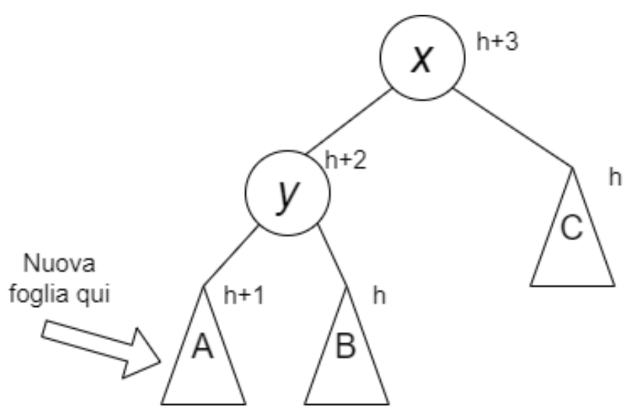
\includegraphics[width=\linewidth]{rotazione 1.1.png}
\end{minipage}
\begin{minipage}{0.1\textwidth}
\hfill
\end{minipage}
\begin{minipage}{0.32\textwidth}
    \centering
    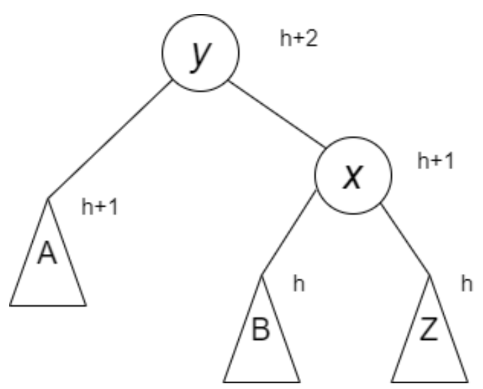
\includegraphics[width=\linewidth]{rotazione 1.2.png}
\end{minipage}

\subsubsection{BF(x)=2 \quad nuovo nodo in x.left.right \quad BF(x.left)=-1}
In questo caso servono 2 rotazioni: una a sinistra sul nodo $y$ e una a destra sul nodo $x$.\\\\
\begin{minipage}{0.31\textwidth}
    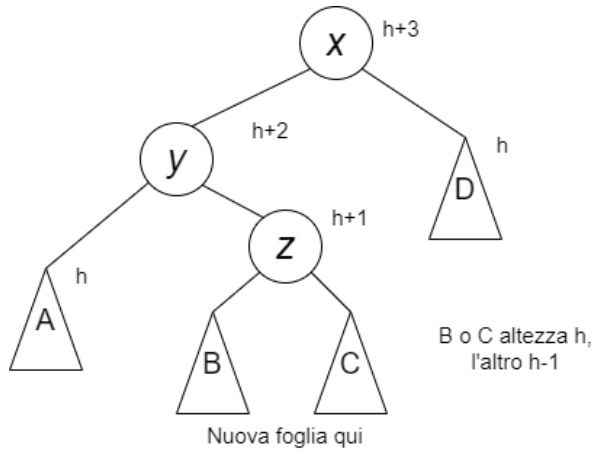
\includegraphics[width=\linewidth]{rotazione 2.1.png}
\end{minipage}
\begin{minipage}{0.31\textwidth}
    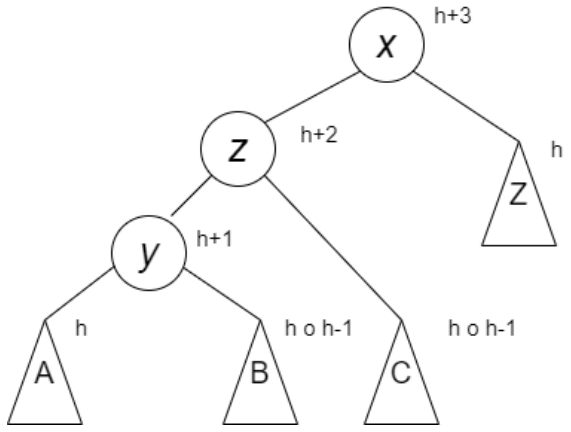
\includegraphics[width=\linewidth]{rotazione 2.2.png}
\end{minipage}
\begin{minipage}{0.38\textwidth}
    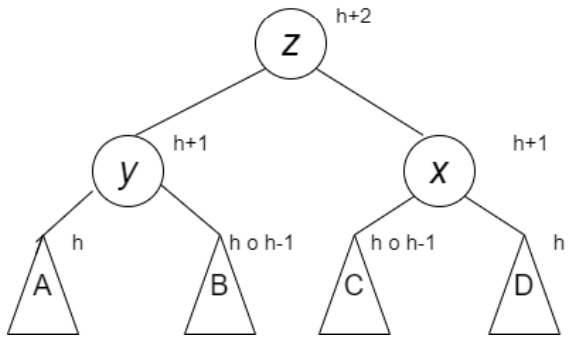
\includegraphics[width=\linewidth]{rotazione 2.3.png}
\end{minipage}

\subsubsection{Algoritmo Fixup}
\textbf{AVL-Insert-Fixup(T,x)}
\begin{algorithmic}[1]
\State $x \leftarrow x.p$
\While{$x \neq T.NIL$}
    \State $x.h \leftarrow \max(x.left.h, x.right.h) + 1$
    \If{$(x.left.h - x.right.h) = 2$} \Comment{BH(x)}
        \If{$(x.left.left.h - x.left.right.h) = -1$} \Comment{BH(x.left)}
            \State Left-Rotate(T, x.left)
        \EndIf
        \State Right-Rotate(T, x)
        \State $x \leftarrow x.p$ \Comment{è ancora radice del sottoalbero, 9-12 simmetrico con 4-7}
    \ElsIf{$(x.left.h - x.right.h) = -2$} \Comment{BH(x)}
        \If{$(x.right.left.h - x.right.right.h) = 1$} \Comment{BH(x.right)}
            \State Right-Rotate(T, x.right)
        \EndIf
        \State Left-Rotate(T, x)
        \State $x \leftarrow x.p$ \Comment{è ancora radice del sottoalbero}
    \EndIf
    \State $x \leftarrow x.p$
\EndWhile
\end{algorithmic}

\subsubsection{Correttezza e Tempo}
Invariante di ciclo: all'inizio di ogni iterazione in AVL c'è al massimo una violazione del bilanciamento.\\
Tempo: 
\begin{itemize}
    \item AVL-Insert $O(lg \, n)$
    \item AVL-Insert-Fixup $O(1)$ per ogni livello, $O(lg \, n)$ livelli $\Rightarrow O(lg \, n)$
\end{itemize}
In totale quindi un inserimento occupa $O(lg \, n)$





























\end{document}
